\chapter{Literature Review}

Several articles have conducted research closely related to ours, 
and will be referenced throughout this chapter: both for their 
theoretical contributions and, in some cases, for data or figures 
that would otherwise have been inaccessible to us.\\

\cite{chang2021videogame_pandemic} examined the impact of COVID-19 
on the amount of time users spent playing video games, drawing data 
from \cite{steamdb} — an independent database covering the entire 
Steam catalog, providing player charts, price history, update 
histories, and detailed product data. Steam itself is the world's 
largest digital distribution platform for PC games, developed by 
Valve Corporation, allowing users to purchase, download, and manage 
games from a centralized library \cite{steam_about}.\\

This article provides a particularly relevant figure, showing 
differences in playtime — across the 500 most popular games at the 
time — between 2019 and 2020.\\

\begin{figure}[H]
    \centering
    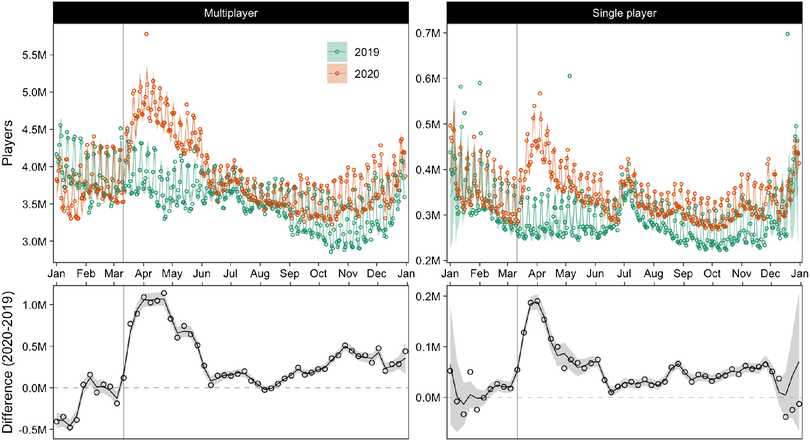
\includegraphics[width=\textwidth]{img/COVID_Steam_Players_Increase.png}
    \caption{Steam players comparison 2019--2020\\
    Note: the vertical gray line marks March 11th, 2020, 
    when the WHO officially declared COVID-19 a pandemic.\\
    Source: \cite{chang2021videogame_pandemic, steamdb}}
    \label{fig:Steam_Players_Increase_COVID1}
\end{figure}
A clear COVID-related effect is visible in the time series, with a 
marked peak between March and May 2020. Notably, the spike in 
multiplayer games persisted longer than that of single-player titles, a pattern that likely reflects users' need to maintain social 
interaction and compensate for the loss of in-person contact during 
lockdown periods.\\
This interpretation finds support in \cite{gaming_disorder_covid}, 
which examined both the adaptive and maladaptive dimensions of video 
game use as a coping strategy during the pandemic. While moderate 
gaming may represent a healthy way to spend time and socialize, excessive use carries the risk of developing into the so-called "gaming disorder". The World Health Organization defines gaming disorder as a pattern of behavior 
characterized by impaired control over gaming, the progressive 
prioritization of gaming over other activities, and its continuation 
despite negative consequences \cite{who_gaming_disorder}. 
\cite{gaming_disorder_covid} further argue that this risk was 
heightened during the pandemic, as many alternative coping 
strategies became unavailable, while opportunities to play -- at any 
hour — increased significantly.\\
The relationship between intensive gaming and mental health is 
explored further in \cite{heavy_gaming&depression}, which finds that 
adolescents classified as heavy gamers reported more depressive 
symptoms than their coetaneous. \cite{gentile2011pathological_gaming} 
refines this picture by highlighting the role of timing, stating that among 
emerging adults aged between 18 and 22 years, habitual late-night gaming (after 2 AM) was associated with heightened vulnerability. This is consistent with \cite{gaming_disorder_covid}'s observation that, as teenagers were free from school schedules (at least at the beginning), they were more likely to extend their gaming sessions into the night.\\
Taken together, this body of literature supports the inclusion of 
depression rates and COVID-related elements (such as Stringency Index) among the variables considered in our analysis, given its documented association with patterns of excessive gaming.

